\documentclass[english]{scrartcl}
\usepackage{setspace}  %% Zur Setzung des Zeilenabstande
\usepackage{calc}      %% ermoeglicht Rechnen mit Laengen und Zaehlern
\usepackage[T1]{fontenc}       %% Unterstutzung von Umlauten etc.
\usepackage[utf8]{inputenc}
\usepackage[utf8]{inputenc}
\usepackage[english]{babel}
\usepackage[english]{isodate}
\usepackage[parfill]{parskip} 
\usepackage{icomma}
\usepackage{listings}
\usepackage{color}
\usepackage[shortlabels]{enumitem}
\usepackage{latexsym,exscale,stmaryrd,amssymb,amsmath}
\usepackage{graphicx}
% Weitere Symbole
\usepackage[nointegrals]{wasysym}
\usepackage{eurosym}
\usepackage{textcomp}
\usepackage{placeins}
\usepackage{wrapfig}
\usepackage{tikz}
\usetikzlibrary{shadows}

\newcommand*\keystroke[1]{%
	\tikz[baseline=(key.base)]
	\node[%
	draw,
	fill=white,
	drop shadow={shadow xshift=0.25ex,shadow yshift=-0.25ex,fill=black,opacity=0.75},
	rectangle,
	rounded corners=1pt,
	inner sep=3pt,
	line width=0.5pt,
	font=\scriptsize\sffamily
	](key) {#1\strut}
	;
}


%opening
\title{User manual - v0.8.0}
\author{by NeoArmageddon}
\titlehead{\centering
\includegraphics[width=12cm]{images/mapbuilder_logo}}
\date{}
\publishers{www.map-builder.info}

\usepackage[
komastyle,
plainfootsepline
]{scrpage2}

\clearscrheadfoot
\ohead[\pagemark]{\pagemark}
\ihead{\leftmark}

\automark[chapter]{section}
\setheadsepline{0.3pt}
\pagestyle{scrheadings}
\usepackage[vmarginratio=1:1, hmarginratio=1:1]{geometry}

\chead[]{\includegraphics[width=0.05\textwidth]{images/Logo.png}}
\cfoot[]{Map Builder User Manual v0.8.0}

%\setheadsepline{0.5pt}[\color{black}]
\setfootsepline{0.5pt}[\color{black}]

\renewcommand*{\titlepagestyle}{empty}
\begin{document}
	
	\maketitle
	\newpage
	\setcounter{secnumdepth}{3} 
	\setcounter{tocdepth}{3} 
	
	\tableofcontents
	\newpage
	\section{Foreword}
	Map Builder is an ingame 3D editor for the game ArmA3 from Bohemia Interactive. Map Builders aim is to assist in the creation of object compositions for terrain creation (export to Terrain Builder), but it can be used for the creation of mission templates (SQM) and object compositions in the form of executable SQF-scripts. Map Builder is \textbf{not} a mission editor. It's sole purpose is the placement and manipulation of static objects.\\
	Map Builder is in Alpha state. That means it is not feature complete and definitly not bug free. But I try to polish every release, so Map Builder can be used in a productive environment.\\
	\\
	What Map Builder \textbf{can't} do:
	\begin{itemize}
		\item Create terrains without Terrain Builder.
		\item Create complete and playready missions.
		\item Place roads.
		\item Generate a terrain with a single button.
	\end{itemize}
	What Map Builder actually \textbf{can} do:
	\begin{itemize}
		\item Accelerate the creation of terrains.
		\item Creates compositions of objects for missions.
		\item Saves you from placing objects with Buldozer!
		\item Allows you to create compositions/terrains with your friends in multiplayer.
	\end{itemize}
	The development of Map Builder began when Bad Benson and ZeroG asked me to create a 3D editor for
	ArmA3 to assist in the placement of objects back in the beginning of 2014. Because of my limited experience with ArmA3's UI design the development slowed down. But in november 2014 I finally pulled myself together, developed an UI framework and made Map Builder useable. From that time on I am continuous working on Map Builder and release updates on a regular base.\\ 
	\newpage
	\section{Installation and Setup}
	The first step is obviously downloading the newest version of Map Builder. If you haven't dine this yet, you can grab the latest version on Armaholic or \textit{www.map-builder.info}. More expierenced users can also grab the latest development build from the official GitHub repository.\\
	After opening the downloaded archive (you need the program \texttt{7zip}) extract the "Map Builder"-folder to a destination of your choice. I recommend your ArmA3 workdir (P:\textbackslash) for this.\\
	In the extracted folder you will find a bunch of other folders:
	\begin{figure}[hb]
		\centering
		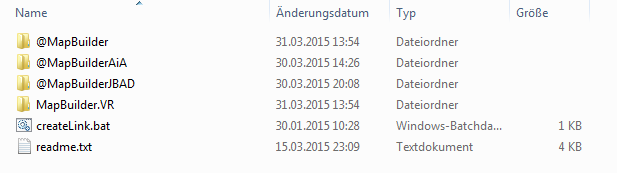
\includegraphics[width=4in]{images/depacked.png}
	\end{figure}
	\FloatBarrier
	The folders with the @-prefix contain the AddOns that unlocks objects in ArmA3 and other AddOns for editor usage. Copy those folders to your ArmA3 game directory (\textit{C:\textbackslash Steam\textbackslash steamapps\textbackslash common\textbackslash Arma 3}) and start them with your favorite way of launching mods (Launcher, param, commandline, ingame...). For basic Map Builder usage you only need to start with \textit{@MapBuilder}. If you want to use Arma1 and Arma2 objects you will also need the \textit{AllInArmA Terrain Pack} and you must include \textit{@MapBuilderAiA} in your startup. For M1lkm8n and Smokedogs JBAD objects you also need \textit{@MapBuilderJBAD} (and obviously JBAD). Please keep in mind that AiA and JBAD will add additional dependencies on your exported compositions (the mod and the MapBuilder upgrade).\\
	\\
	The core of Map Builder is packed as a mission. For basic usage you can copy the \textit{MapBuilder.VR} folder to your ArmA3 mission directory (\textit{C:\textbackslash Users\textbackslash Username\textbackslash Documents\textbackslash Arma 3 - Other Profiles\textbackslash Nickname\textbackslash missions}). You can rename the mission and change the terrain suffix to port the mission to another terrain (for example renaming it to \textit{MapBuilder.Stratis} allows you to use Map Builder on Stratis).\\
	You can also use the \textit{createlink.bat} file. It will ask you for your mission directory and the island you want Map Builder on. It will then create a symbolic link to the MapBuilder.VR mission. This means you have the mission only once on your disc but you can have it on multiple terrains.\\
	\\
	Now you can launch ArmA3, start the ingame 2D editor, select the Map Builder mission, load it (maybe you need to move the player units onto land) and preview it. When previewing you can click \textit{"Start Map Builder"} in the action menu and Map Builder will open.
	\section{Userinterface}
	After launching Map Builder you will be presented with the Map Builder UI.
	\begin{figure}[hb]
		\centering
		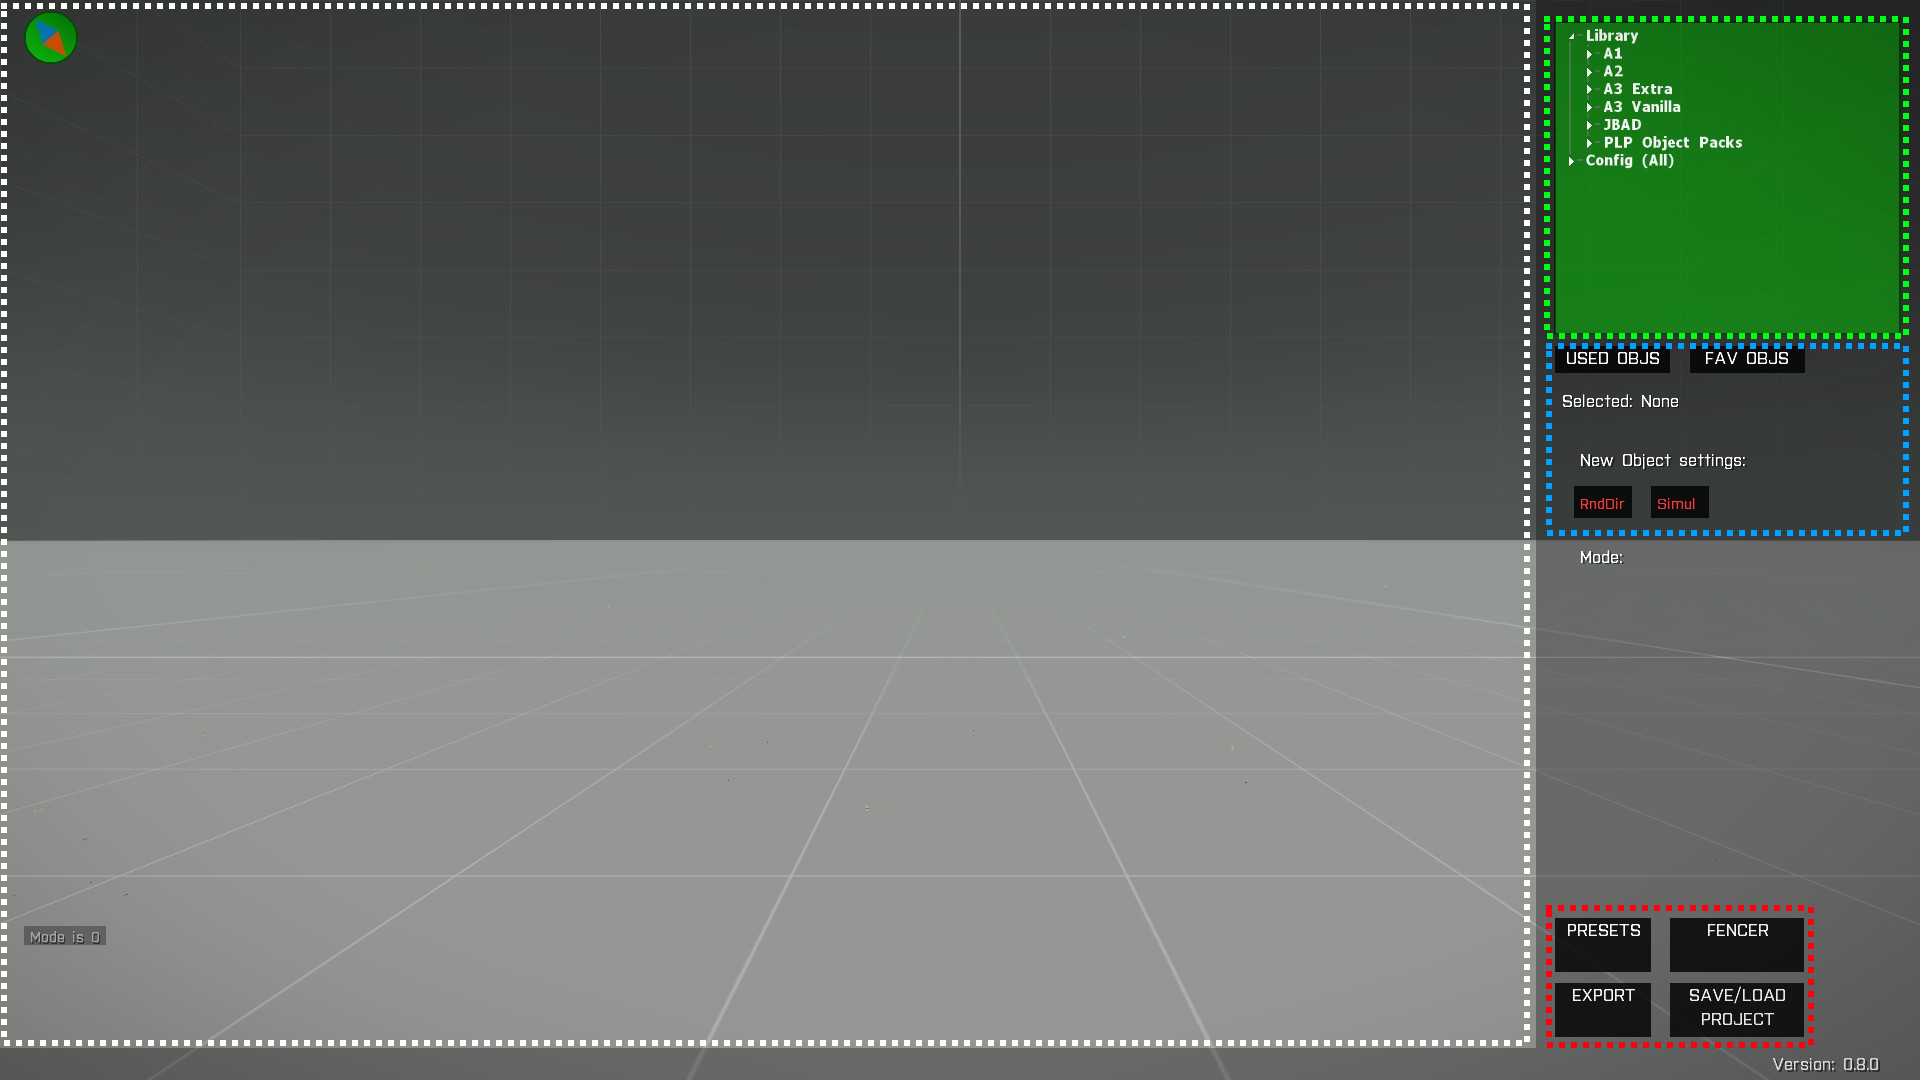
\includegraphics[width=5.8in]{images/mb/mbui.png}
	\end{figure}
	\FloatBarrier
	The area marked with the white box is the \textbf{main viewport}. This is were you will interact with the objects on the map. Only when the viewport has focus (mouse is in the viewport) you are able to click objects and move through the world.\\
	\\
	On the right side you will find the \textbf{object library} (green box) were you can browse all loaded objects. All objects are sorted in categories. At the highest level you have the \textit{Library} and the \textit{Config (All)} nodes. The \textit{Library} node contains all "Map Builder objects". That are objects that are known to be placeable in Map Builder. With the @MapBuilder AddOn you will have access to all of ArmA3's static objects like buildings, signs, fortification, etc (basically everything that can be placed in the 2D editor or Zeus).You find all of those objects under "A3 Vanilla". You will also have the options to place objects that are not placeable in vanilla ArmA3. Those are objects like rocks, bushes and trees. They are located in "Library -> A3 Extra". Be aware that those "extra" objects add a additional addon dependency for \textit{@MapBuilder} to your exported compositions. When you only use objects from "A3 Vanilla" your exports can be used anywhere without additional addons.\\
	When you have the AllInArmA terrain pack, JBAD and the corresponding MapBuilder addons enabled, you will have access to even more categories like "A1","A2" and "JBAD".\\
	When selecting an objects a 3D preview will open, so you can inspect the object before placing it.\\
	Some addons may add themself to your library (for example \textit{Poolpunk's beach objects}). If you are an AddOn developer have a look at chapter XXX to learn how to add your own AddOns to the Map Builder library.\\
	\\
	In the blue box you can find the buttons to open a list of all used objects and the list of favored objects. Underneath you find the current selected object and two switches that affect how objects are placed. The first switch \textit{RndDir} toggles the random orientation, when placing objects. The \textit{Simul} switch toggles simulation of placed objects. When you are placing vehicles you want this to be enabled. Otherweise you won't be able to get in the vehicles and physics won't affect them. When you are placing objects like walls, trees, houses and furniture you want this to be disabled so physics don't act on them (especially furniture tend to jump around).\\
	\\
	In the red box you find all buttons to access the advanced function of Map Builder:
	\begin{itemize}
		\item \textbf{Presets} - Here you can save and load small compositions of objects (presets) that can be moved around free.
		\item \textbf{Fencer} - Fencer assists in placing lines of objects (like fences).
		\item \textbf{Export} - Here you can export your current objects to Terrain Builder, SQM and SQF.
		\item \textbf{Save/Load project} - Here you can save and load your project. You can also reset the current project and import another project in the current one.
	\end{itemize}
	Some buttons may open new windows. Most of those windows can be moved free across the screen.\\
		\begin{figure}[hb]
			\centering
			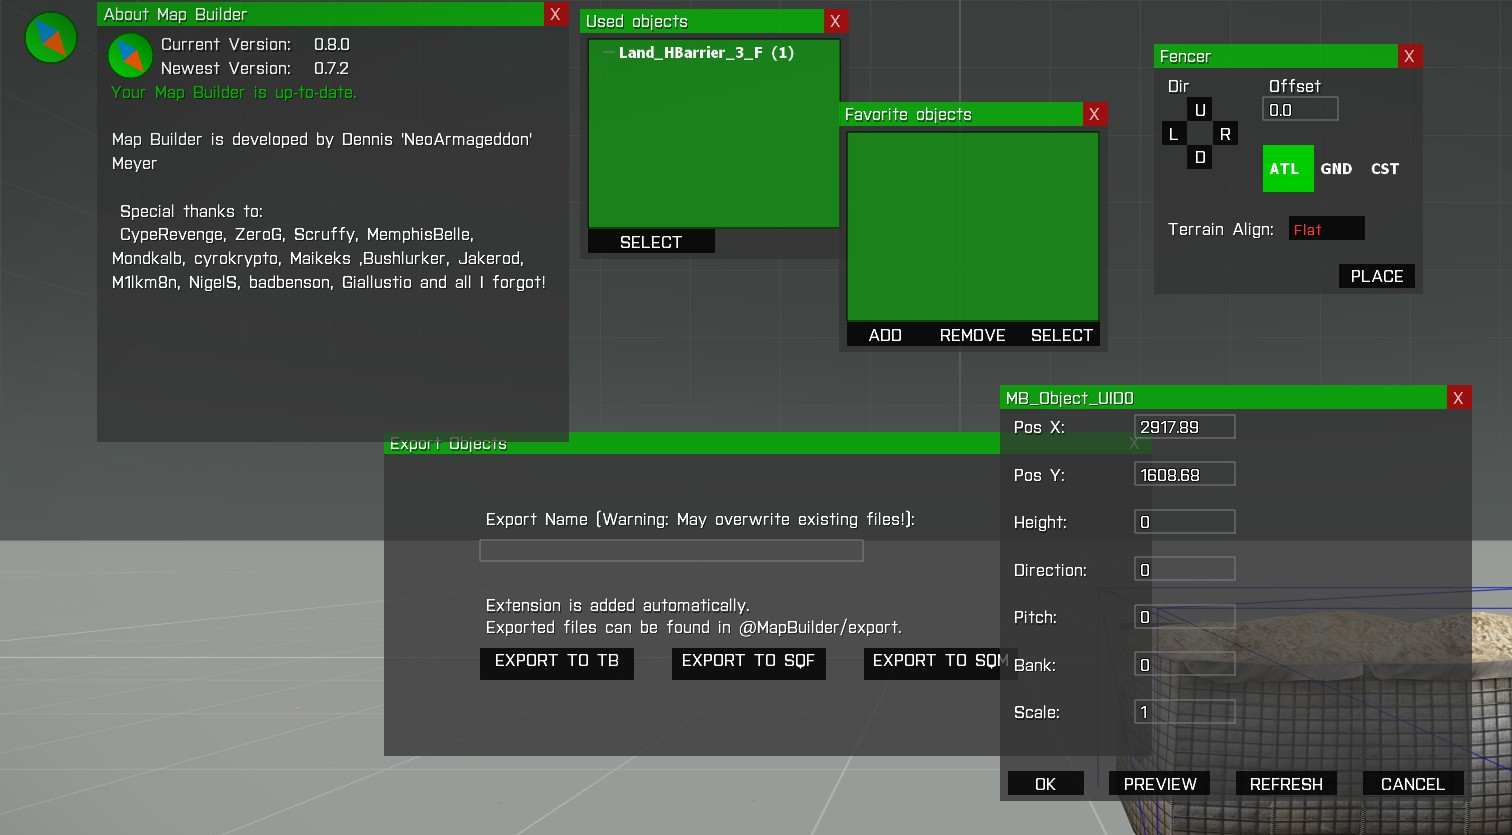
\includegraphics[width=5.8in]{images/mb/windows.png}
		\end{figure}
		\FloatBarrier
	\newpage
	\section{Movement}
	First make sure you the main viewport has focus (the mouse is in it and not ontop of a popup window)!\\
	You can move the Map Builder camera around by pressing \keystroke{W},\keystroke{A},\keystroke{A} and \keystroke{D}.
	With \keystroke{Q} and \keystroke{Z} you can move the camera up and down. Pressing \keystroke{Shift} while moving will make
	the camera move faster. \keystroke{Left Alt} will make it even faster. \\	
	With the \keystroke{Num}-keys you can rotate the camera.\\
	When holding the middle mouse button you can look around with the mouse.\\
	The mouse scrollwheel will zoom the camera in and out.
	\newpage
	\section{Basic Object Manipulation}
	After selecting an objects from the library you can double left click on the terrain in the viewport to create a new object. It will be selected right away indicated by a blue bounding box.
		\begin{figure}[hb]
			\centering
			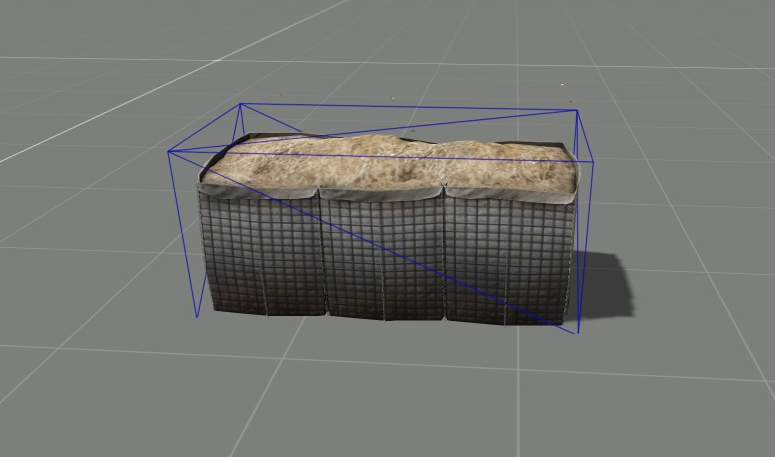
\includegraphics[width=3.8in]{images/mb/selection.png}
		\end{figure}
		\FloatBarrier
	You can deselect the objects by clicking somewhere on the terrain and reselecting the object by clicking on it.
	When you hold the \keystroke{Shift} key you can select multiple objects at the same time. You can also hold down the left mouse button somewhere on the terrain and drag a selection rectangle to select a bunch of objects.
	\begin{figure}[hb]
		\centering
		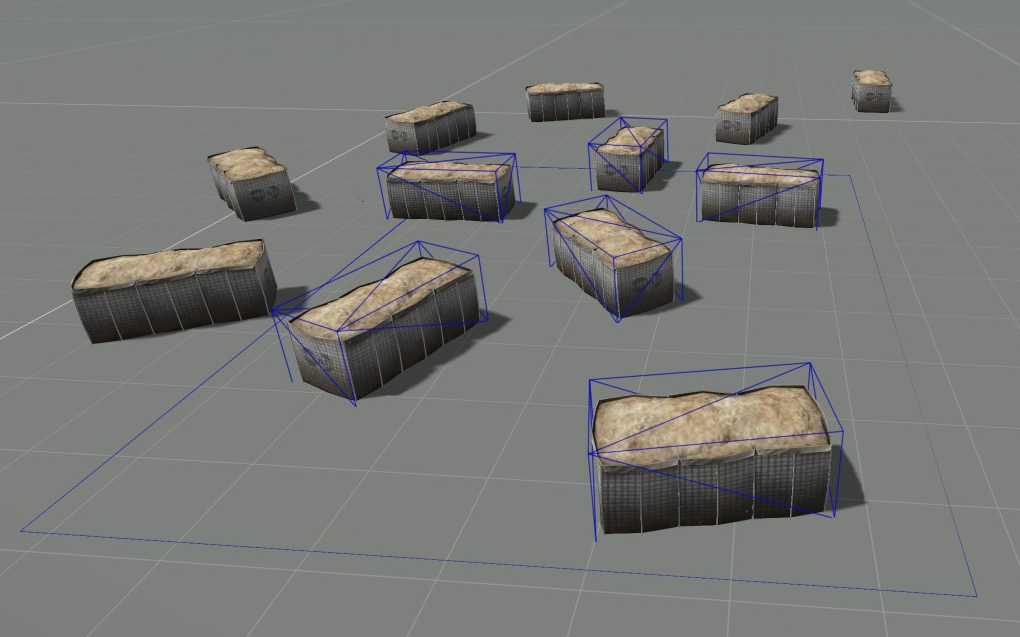
\includegraphics[width=4.8in]{images/mb/selectionrectangle.png}
	\end{figure}
	\FloatBarrier 
	Be aware that only objects with a geometry can be clicked. All other objects can only be selected by drawing a selectionrectangle.\\
	To move a selection of objects around, just hold down the left mouse button and move the mouse over the terrain.
	As the objects are moved in relation to the mouse movement on the terrain, the objects will move faster if you drag them towards the horizon. This may first seem unnatural but you will get the grip of it very quick. Objects are best handled from a camera position above the objects (like a isometric camera).\\
	You can rotate one or more objects by holding down the right mouse button and moving the mouse. The center of rotation is the center of one objects or the center of mass of multiple objects. When you hold down \keystroke{Shift} the center of rotation will be the point your mouse is pointing at.\\
	You can change the height of objects when you hold down both left and right mouse button and move the mouse. When moving an object up you will notice a line going to the ground. This indicated the position of a floating objects. When moving floating objects you best drag it from the point this line is intersecting the ground so you won't be affected by the viewport projection (you will see what I mean when you grap a floating object from it's visual position).\\
	\\
	When holding down \keystroke{Ctrl}and pressing down the left mouse button you can change the pitch of selected objects. With the right mouse button you can change the bank.\\
	\\
	\begin{wrapfigure}{r}{0.44\textwidth}
		\begin{center}
			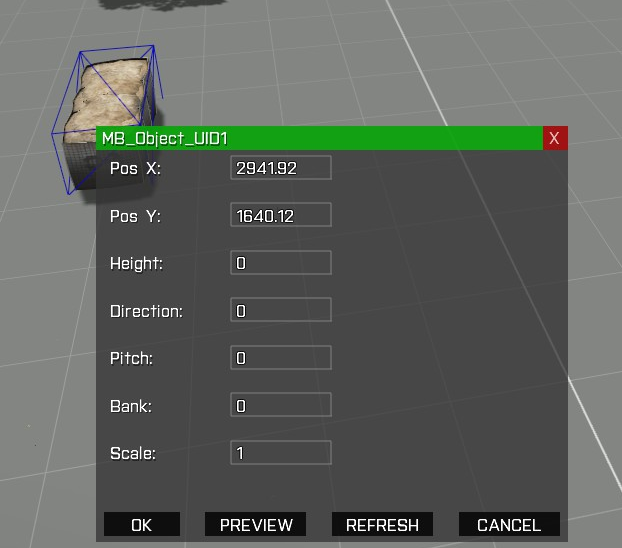
\includegraphics[width=0.42\textwidth]{images/mb/inspector.png}
		\end{center}
	\end{wrapfigure}
	You can finetune an objects properties by double right click on an object. The objectinspector window will open. You can change all object properties from here. Pressing "Ok" will apply all changes to the object. "Preview" will apply the changes but without actually saving them. So you can preview the changes. When you want to revert an object, just press "Cancel". The objectinspector window is not updated, when you move an inspected object in the viewport. Press "Refresh" to copy the new values into the window.\\
	\\
	You can reset an objects rotation, pitch and bank by selecting the object and pressing \keystroke{Ctrl}+\keystroke{R}.\\
	You can also align objects to the terrain by pressin \keystroke{Ctrl}+\keystroke{T}.\\
	\\
	Objectselection can be copy and pasted (\keystroke{Ctrl}+\keystroke{C} and \keystroke{Ctrl}+\keystroke{V}).
	%\section{Fencer}
	%\section{Presets}
	%\section{Projects}
	%\section{Export}
	%section{Multiplayer}
	%section{Support}
	%\section{Control Cheat Sheet}
	%\section{Credits}
\end{document}